\sectionframe{Feature Distribution Smoothing (FDS)}

\begin{frame}{Feature statistics similarity for anchor age 0}
	\begin{figure}[h]
		\begin{subfigure}{0.48\textwidth}
			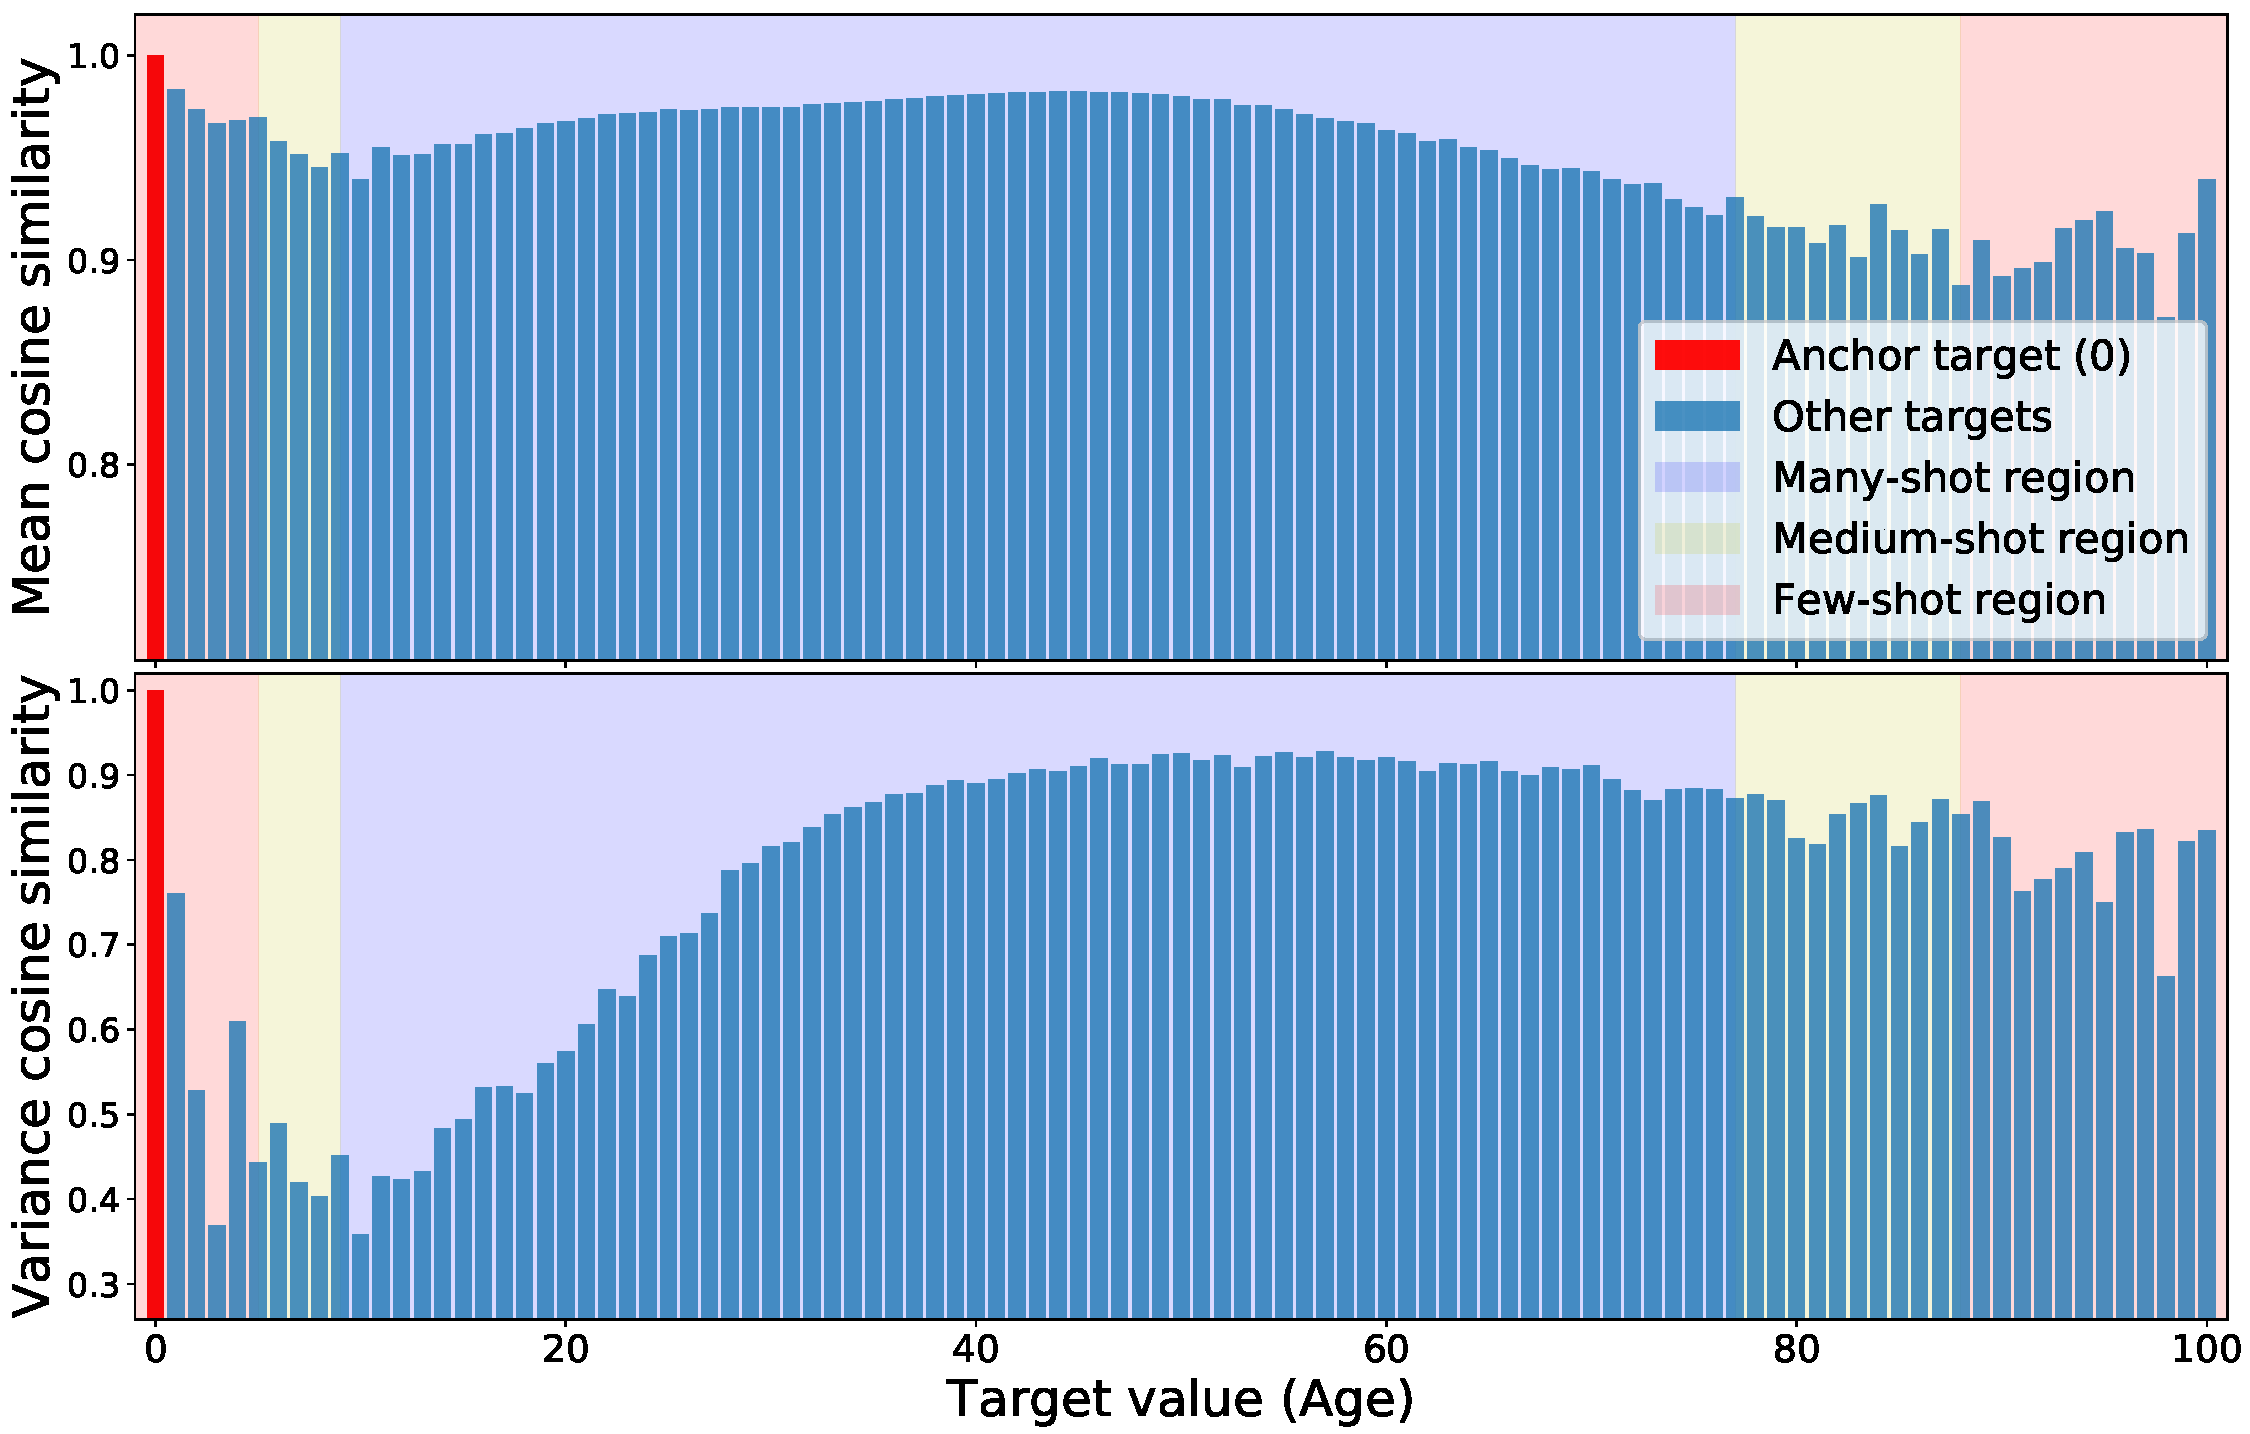
\includegraphics[width=\linewidth]{images/feat_sim_fds_base_0.pdf}
			\caption{Baseline}
		\end{subfigure}\hspace{1em}%
		\begin{subfigure}{0.48\textwidth}
			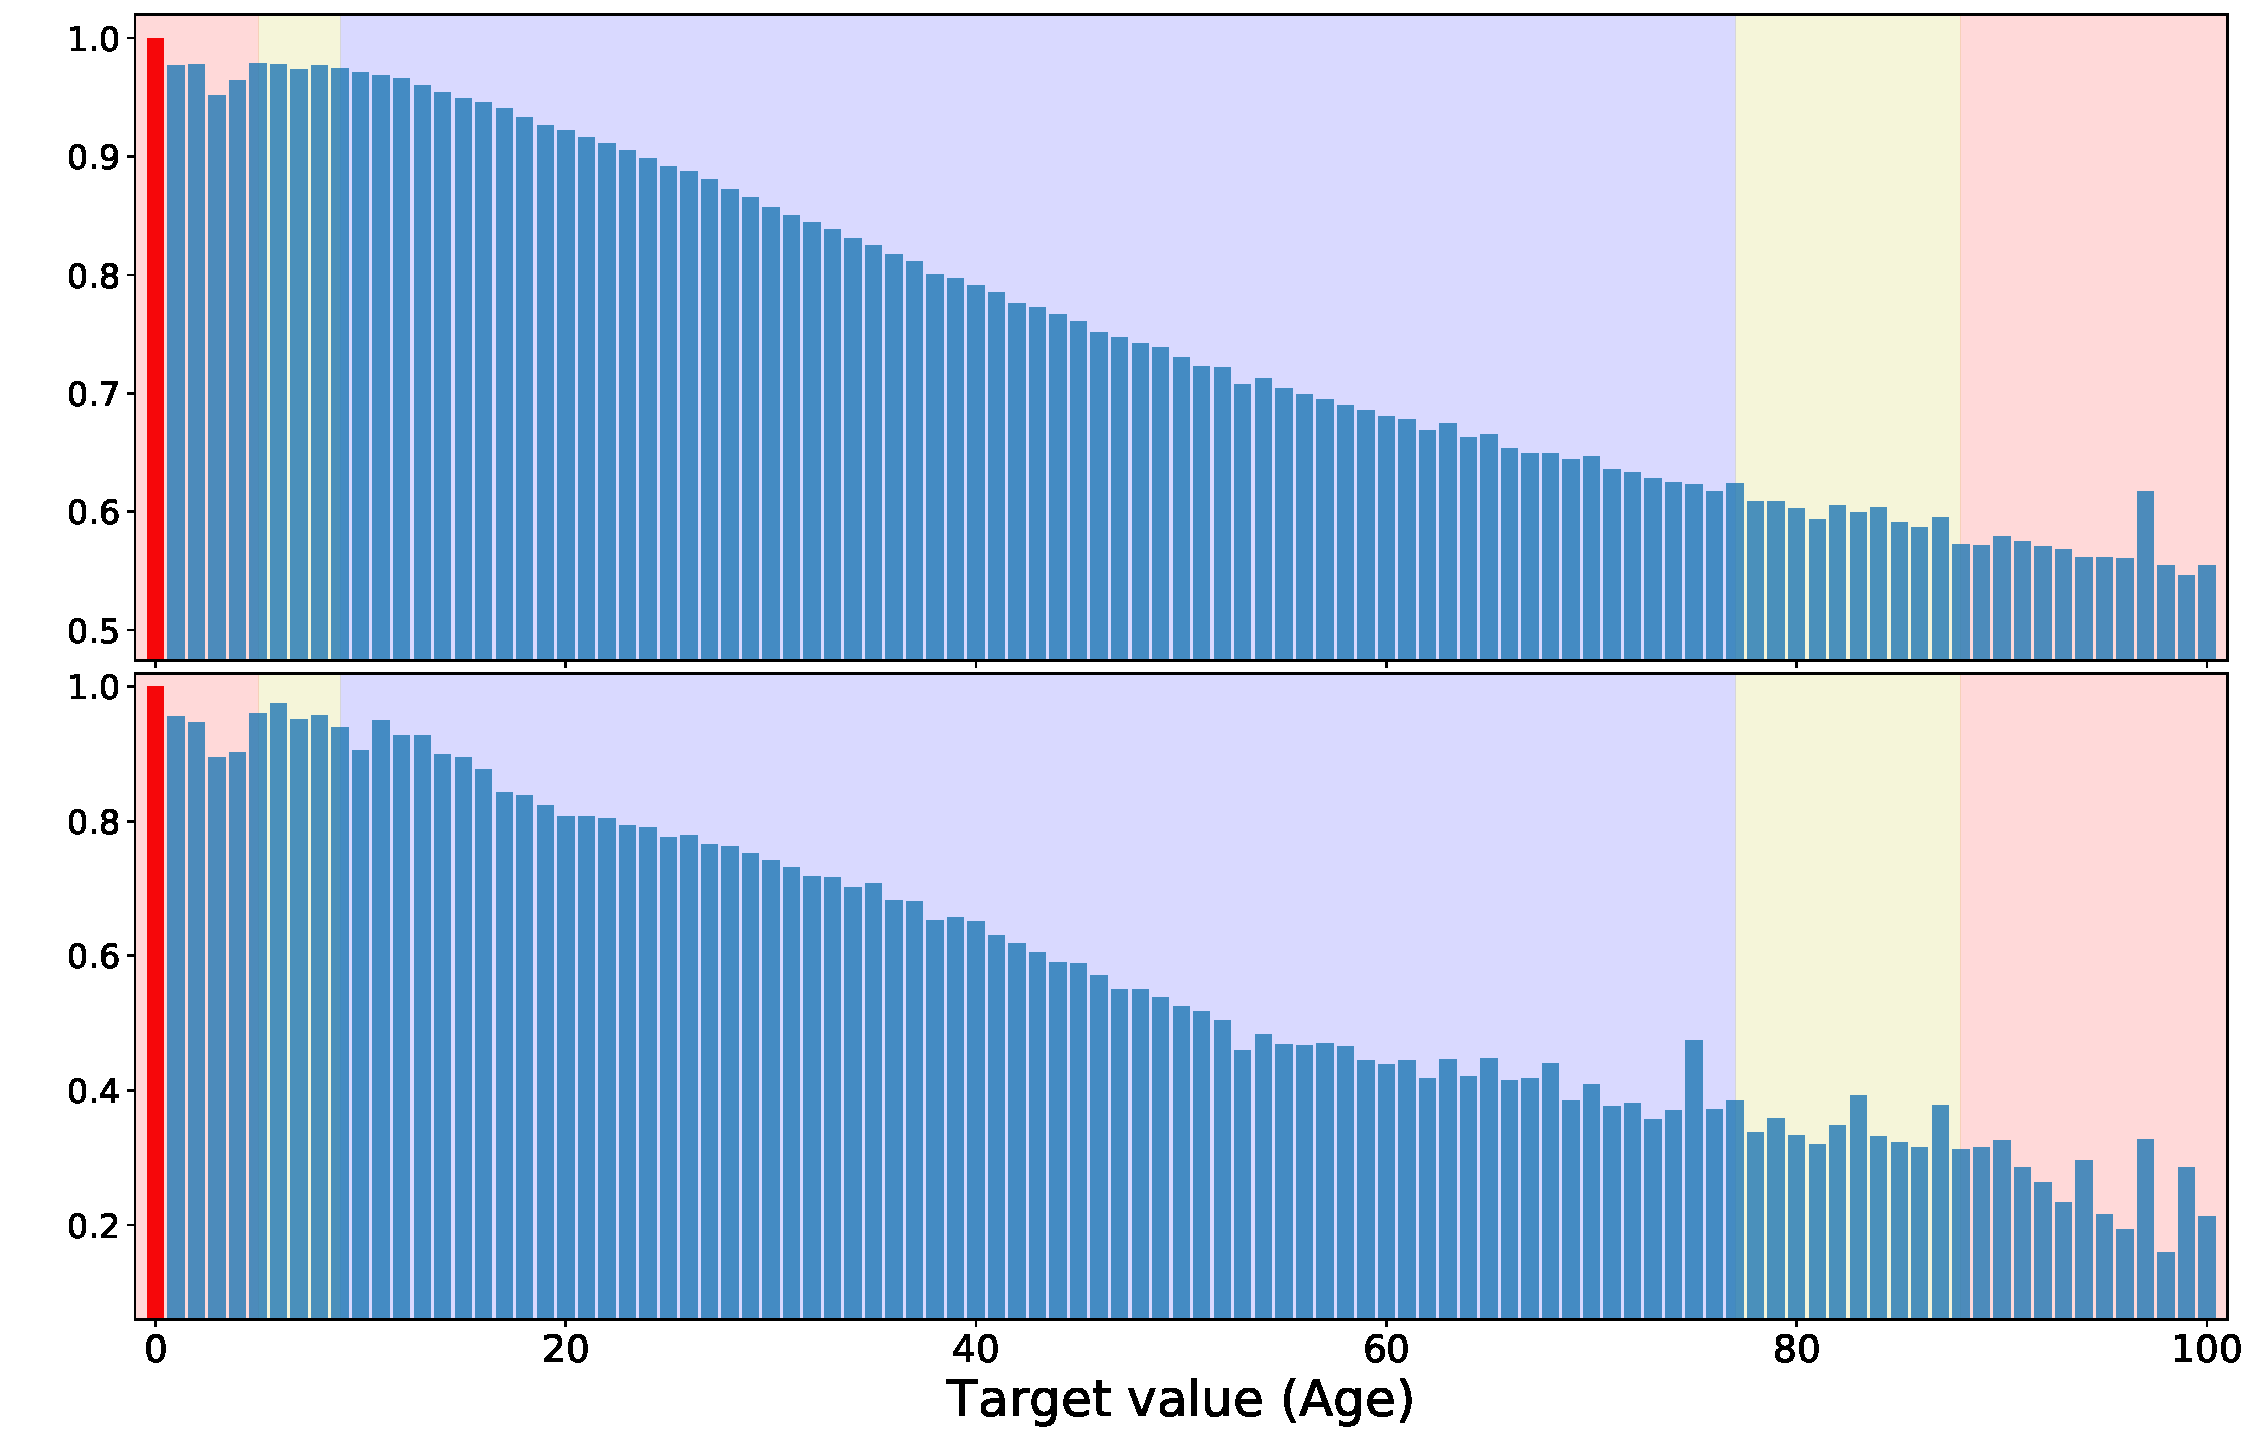
\includegraphics[width=\linewidth]{images/feat_sim_fds_ours_0.pdf}
			\caption{FDS}
		\end{subfigure}
		%\caption{}
	\end{figure}
	\begin{itemize}
		\item FDS improves feature statistics calibration:
		\begin{itemize}
			\item High similarity only in neighbourhood
			\item Gradually decreasing similarity as the target becomes smaller or larger
		\end{itemize}
	\end{itemize}
	\credit{Image}{yang2021delving}
\end{frame}

\begin{frame}{Feature statistics similarity for anchor age 30}
	\begin{figure}[h]
		\begin{subfigure}{0.48\textwidth}
			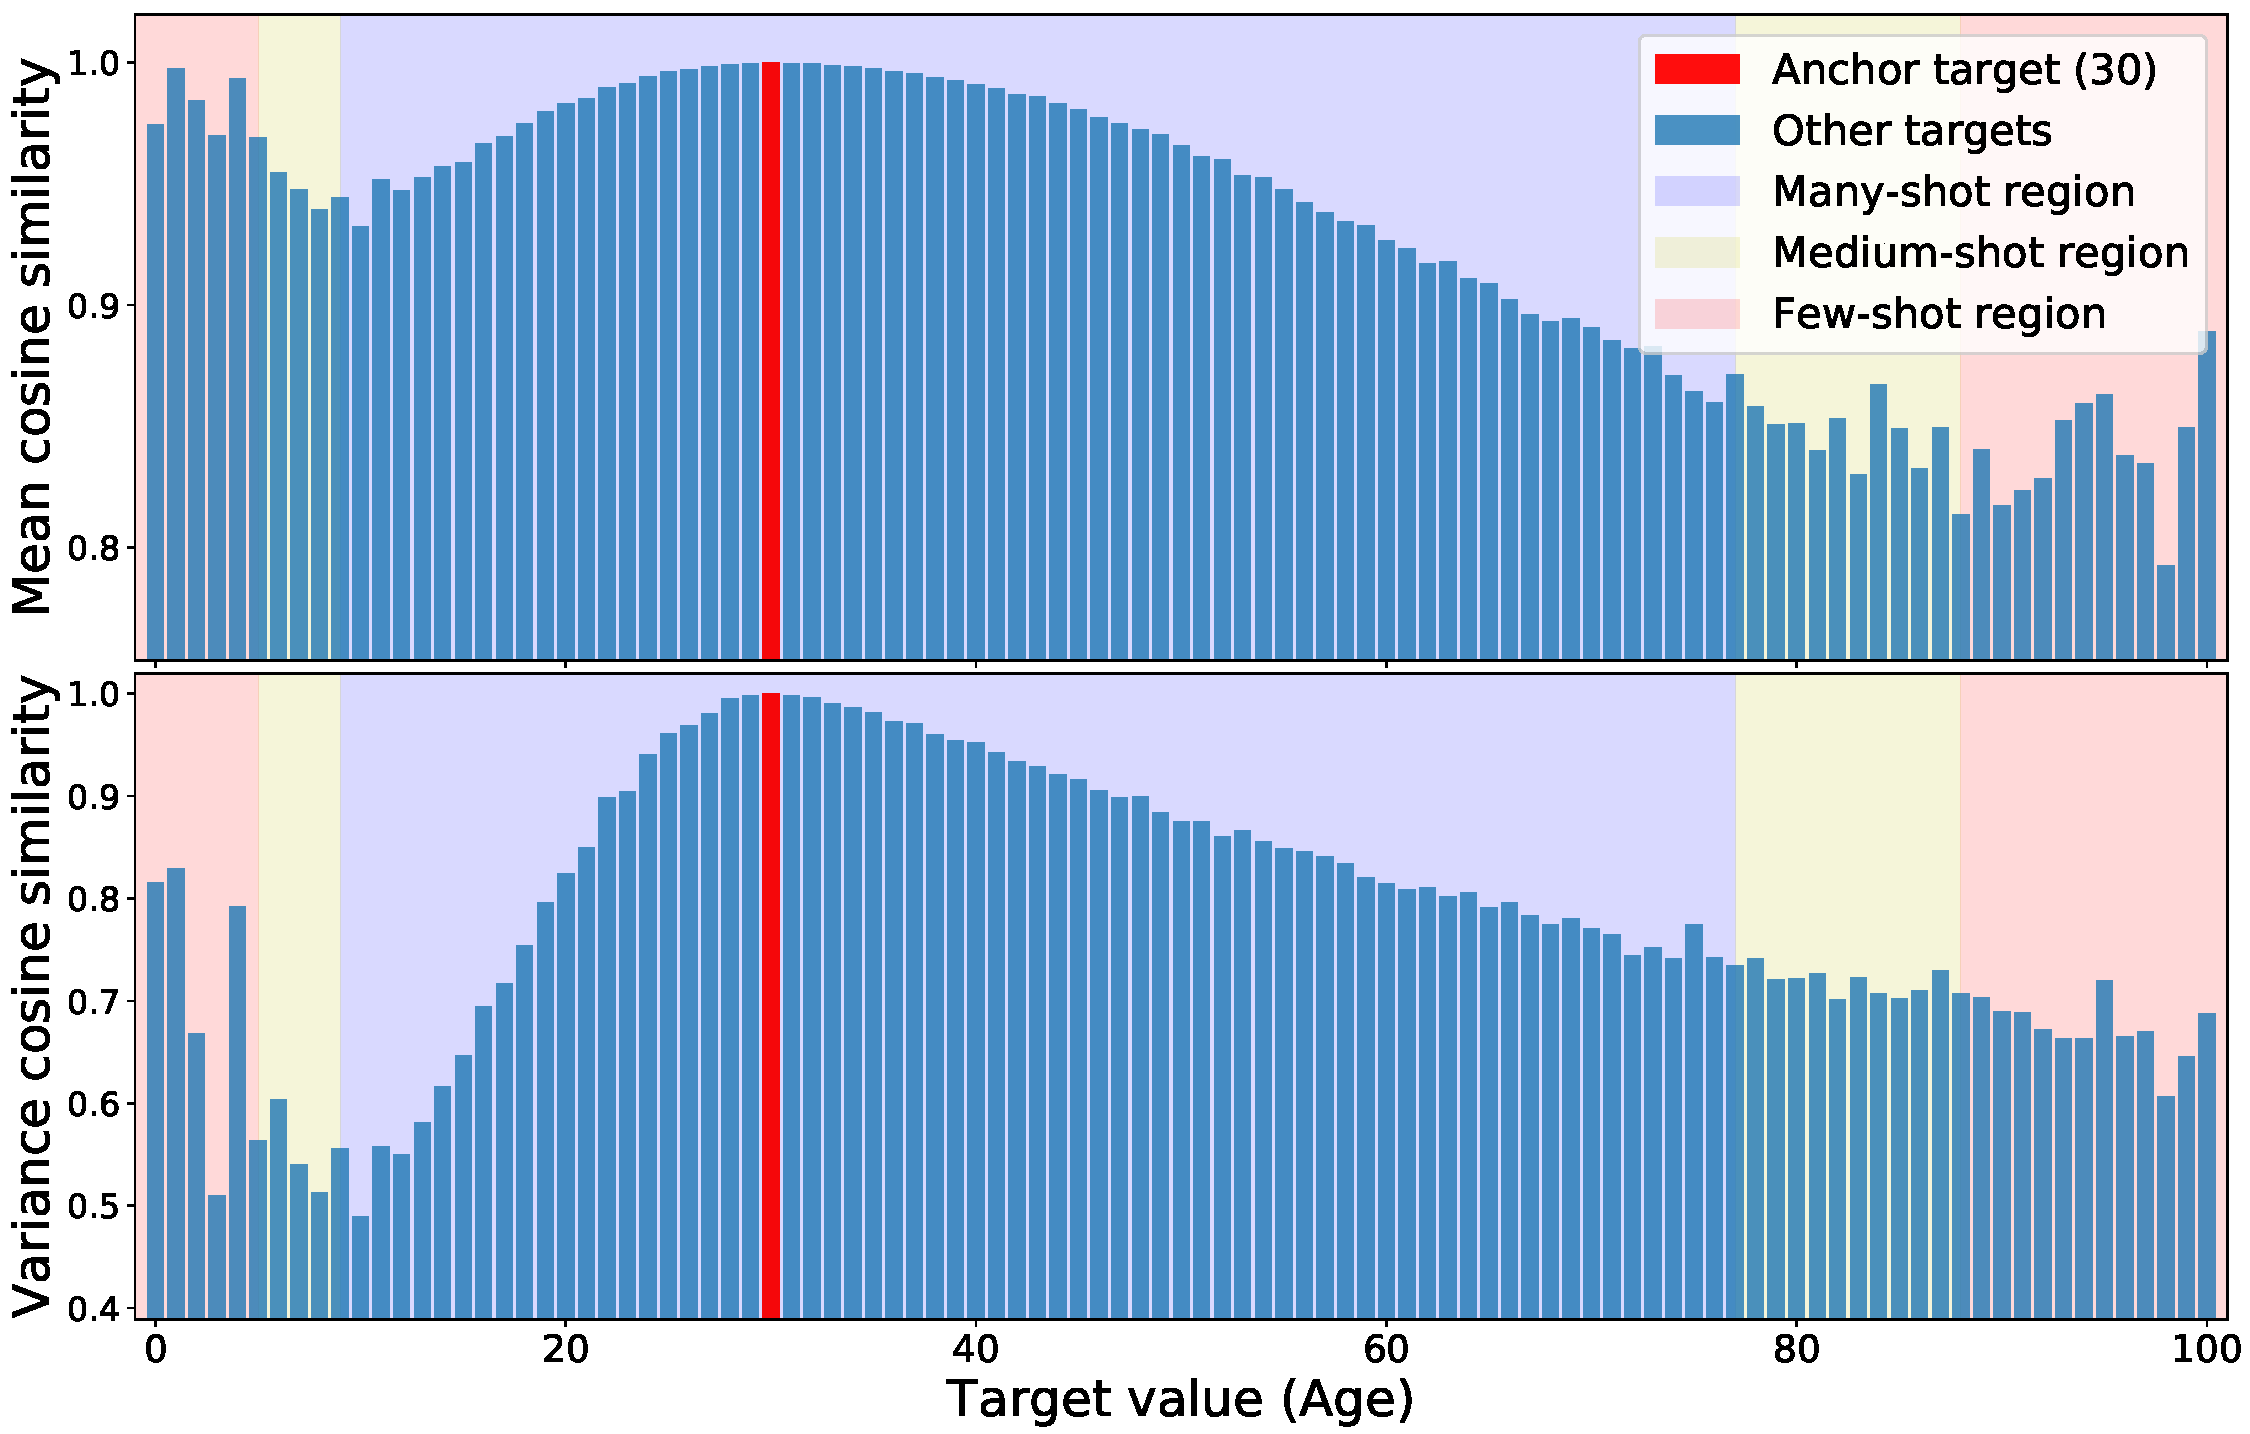
\includegraphics[width=\linewidth]{images/feat_sim_fds_base_30.pdf}
			\caption{Baseline}
		\end{subfigure}\hspace{1em}%
		\begin{subfigure}{0.48\textwidth}
			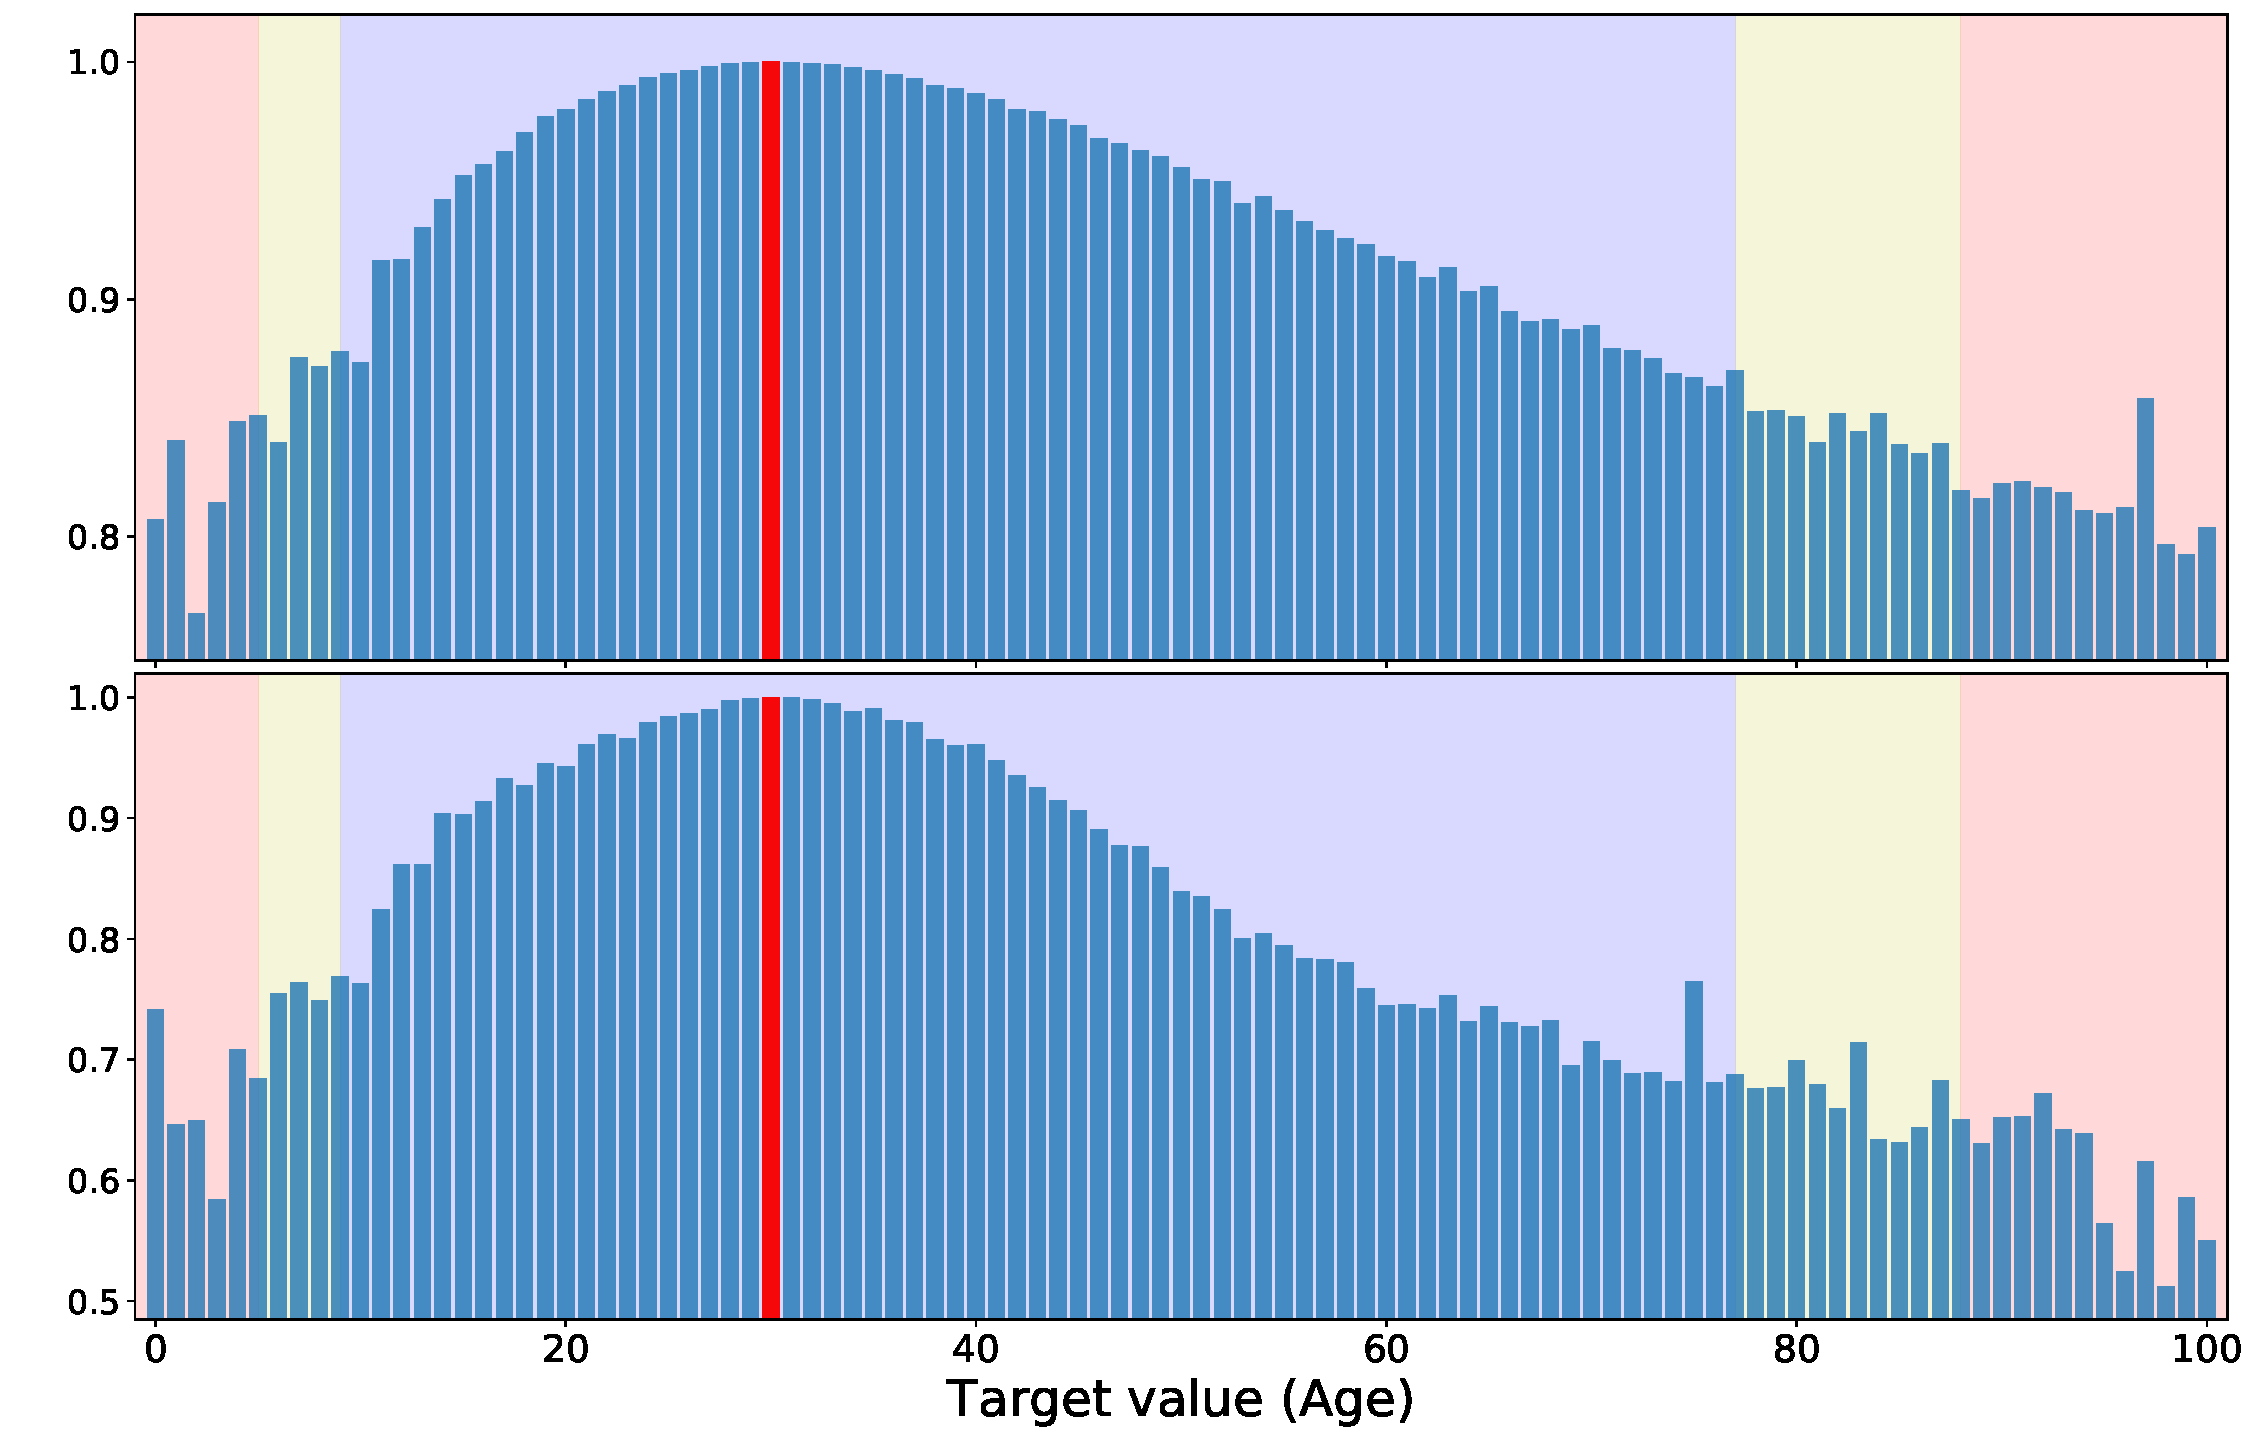
\includegraphics[width=\linewidth]{images/feat_sim_fds_ours_30.pdf}
			\caption{FDS}
		\end{subfigure}
		%\caption{}
	\end{figure}
	\begin{itemize}
		\item FDS improves feature statistics calibration:
		\begin{itemize}
			\item High similarity only in neighbourhood
			\item Gradually decreasing similarity as the target becomes smaller or larger
		\end{itemize}
	\end{itemize}
	\credit{Image}{yang2021delving}
\end{frame}

\begin{frame}{Feature statistics similarity for anchor age 60}
	\begin{figure}[h]
		\begin{subfigure}{0.48\textwidth}
			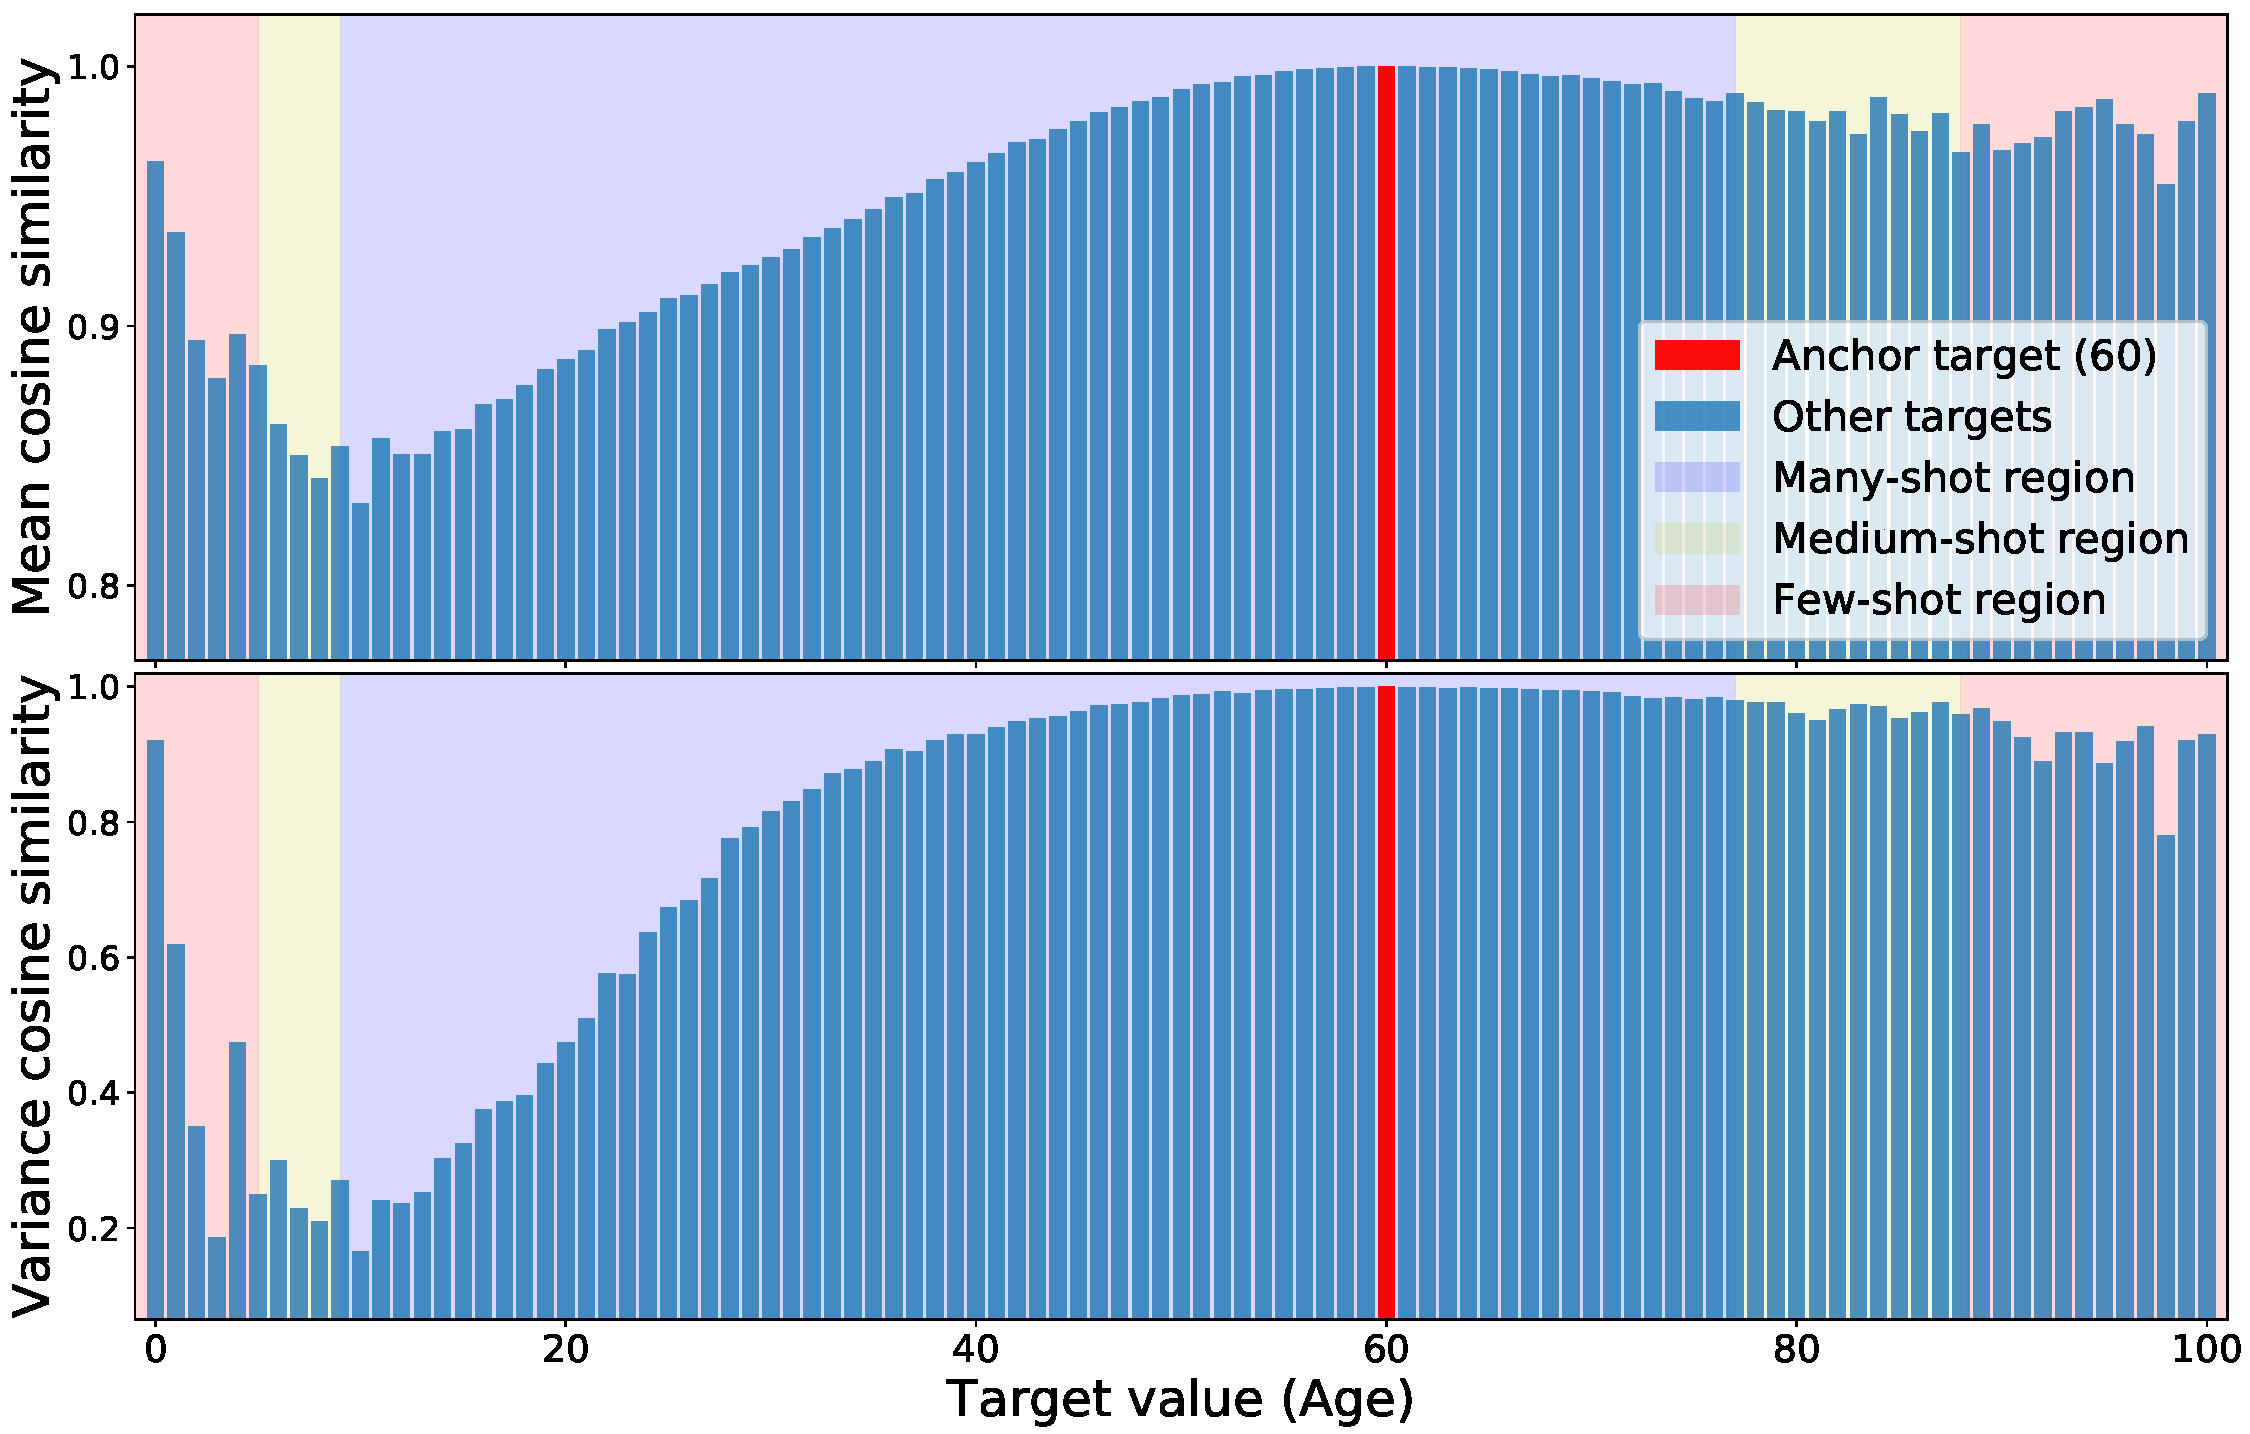
\includegraphics[width=\linewidth]{images/feat_sim_fds_base_60.pdf}
			\caption{Baseline}
		\end{subfigure}\hspace{1em}%
		\begin{subfigure}{0.48\textwidth}
			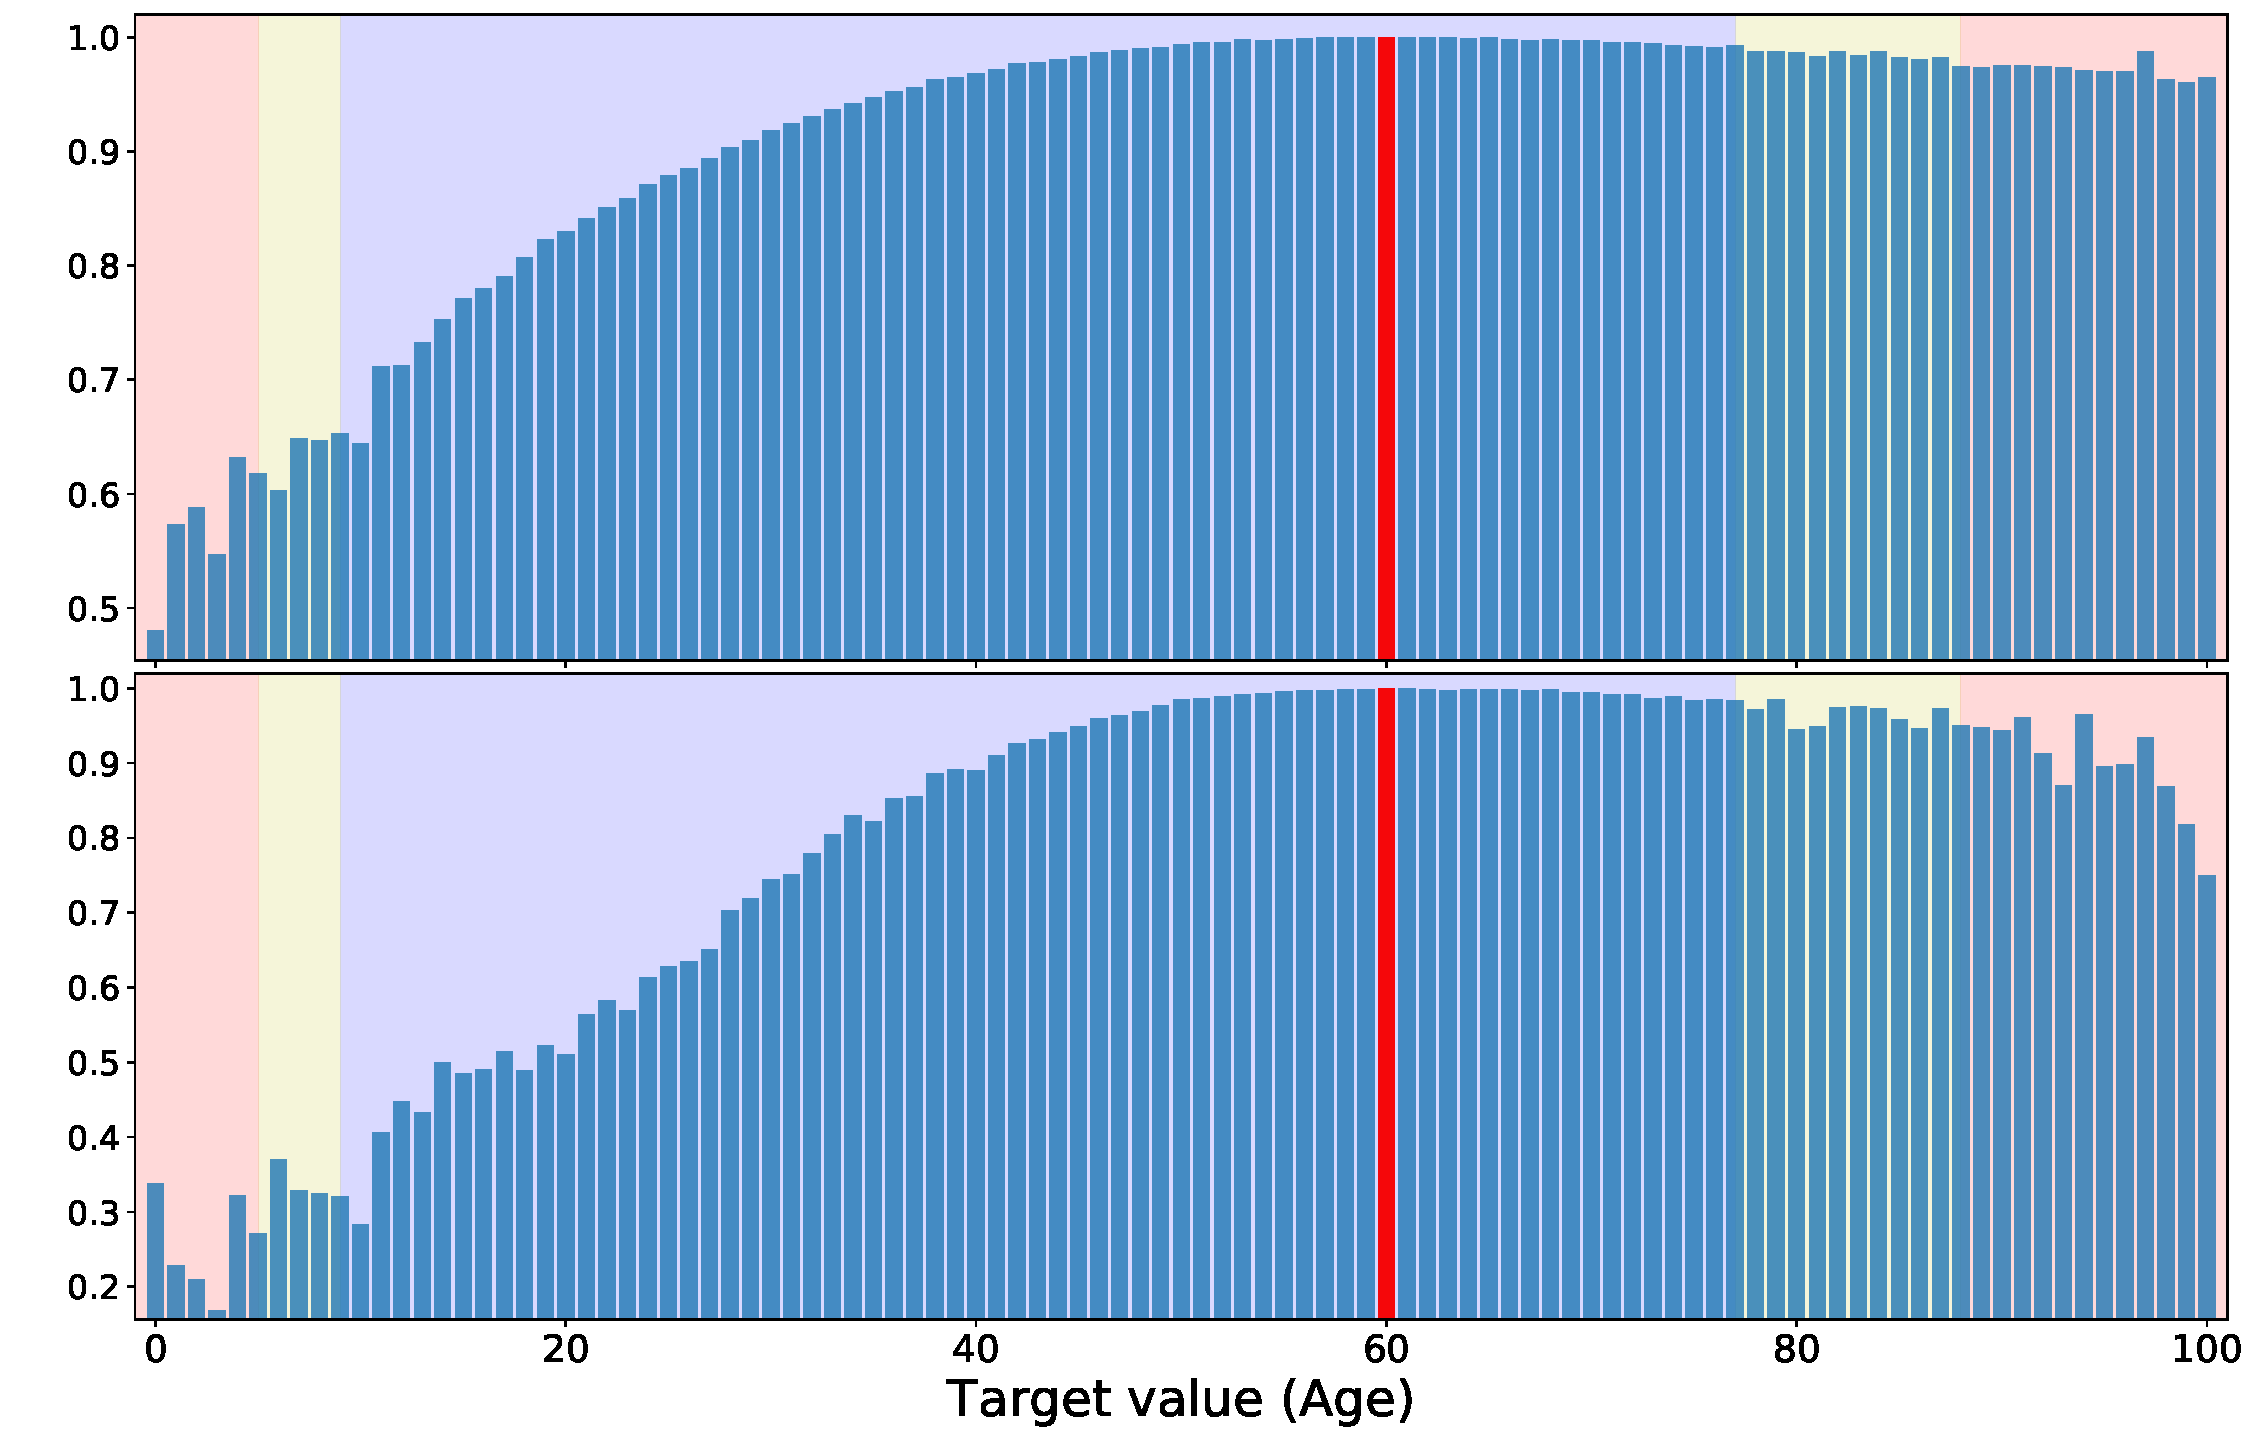
\includegraphics[width=\linewidth]{images/feat_sim_fds_ours_60.pdf}
			\caption{FDS}
		\end{subfigure}
		%\caption{}
	\end{figure}
	\begin{itemize}
		\item FDS improves feature statistics calibration:
		\begin{itemize}
			\item High similarity only in neighbourhood
			\item Gradually decreasing similarity as the target becomes smaller or larger
		\end{itemize}
	\end{itemize}
	\credit{Image}{yang2021delving}
\end{frame}

\begin{frame}{Feature statistics similarity for anchor age 90}
	\begin{figure}[h]
		\begin{subfigure}{0.48\textwidth}
			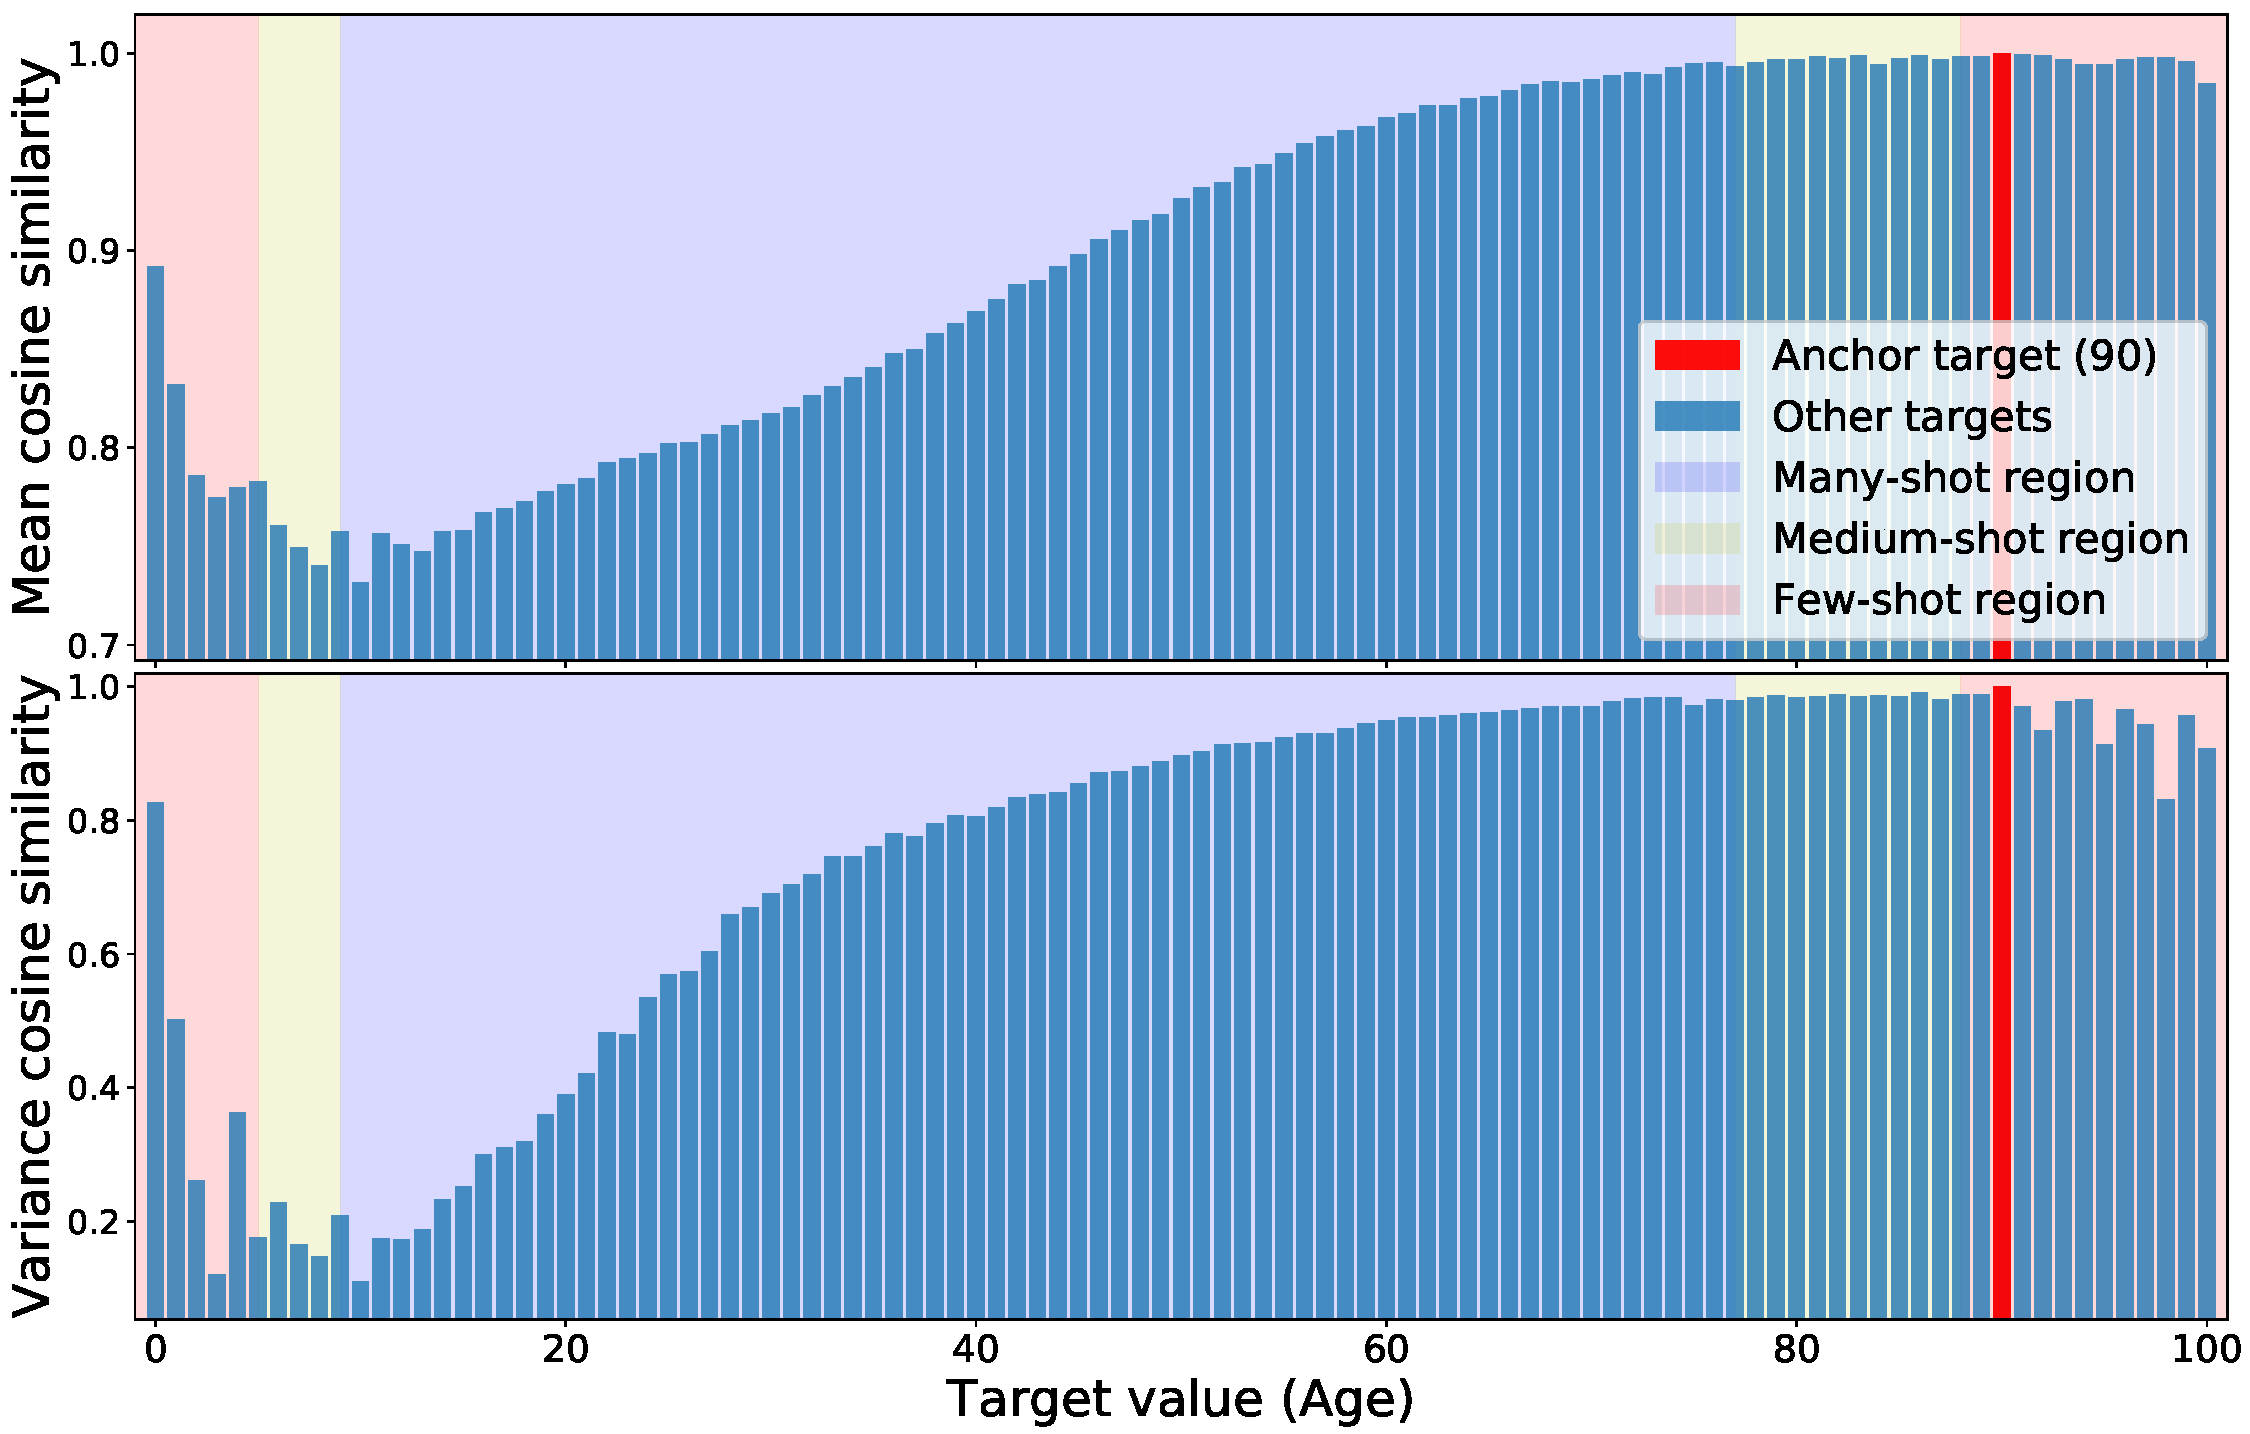
\includegraphics[width=\linewidth]{images/feat_sim_fds_base_90.pdf}
			\caption{Baseline}
		\end{subfigure}\hspace{1em}%
		\begin{subfigure}{0.48\textwidth}
			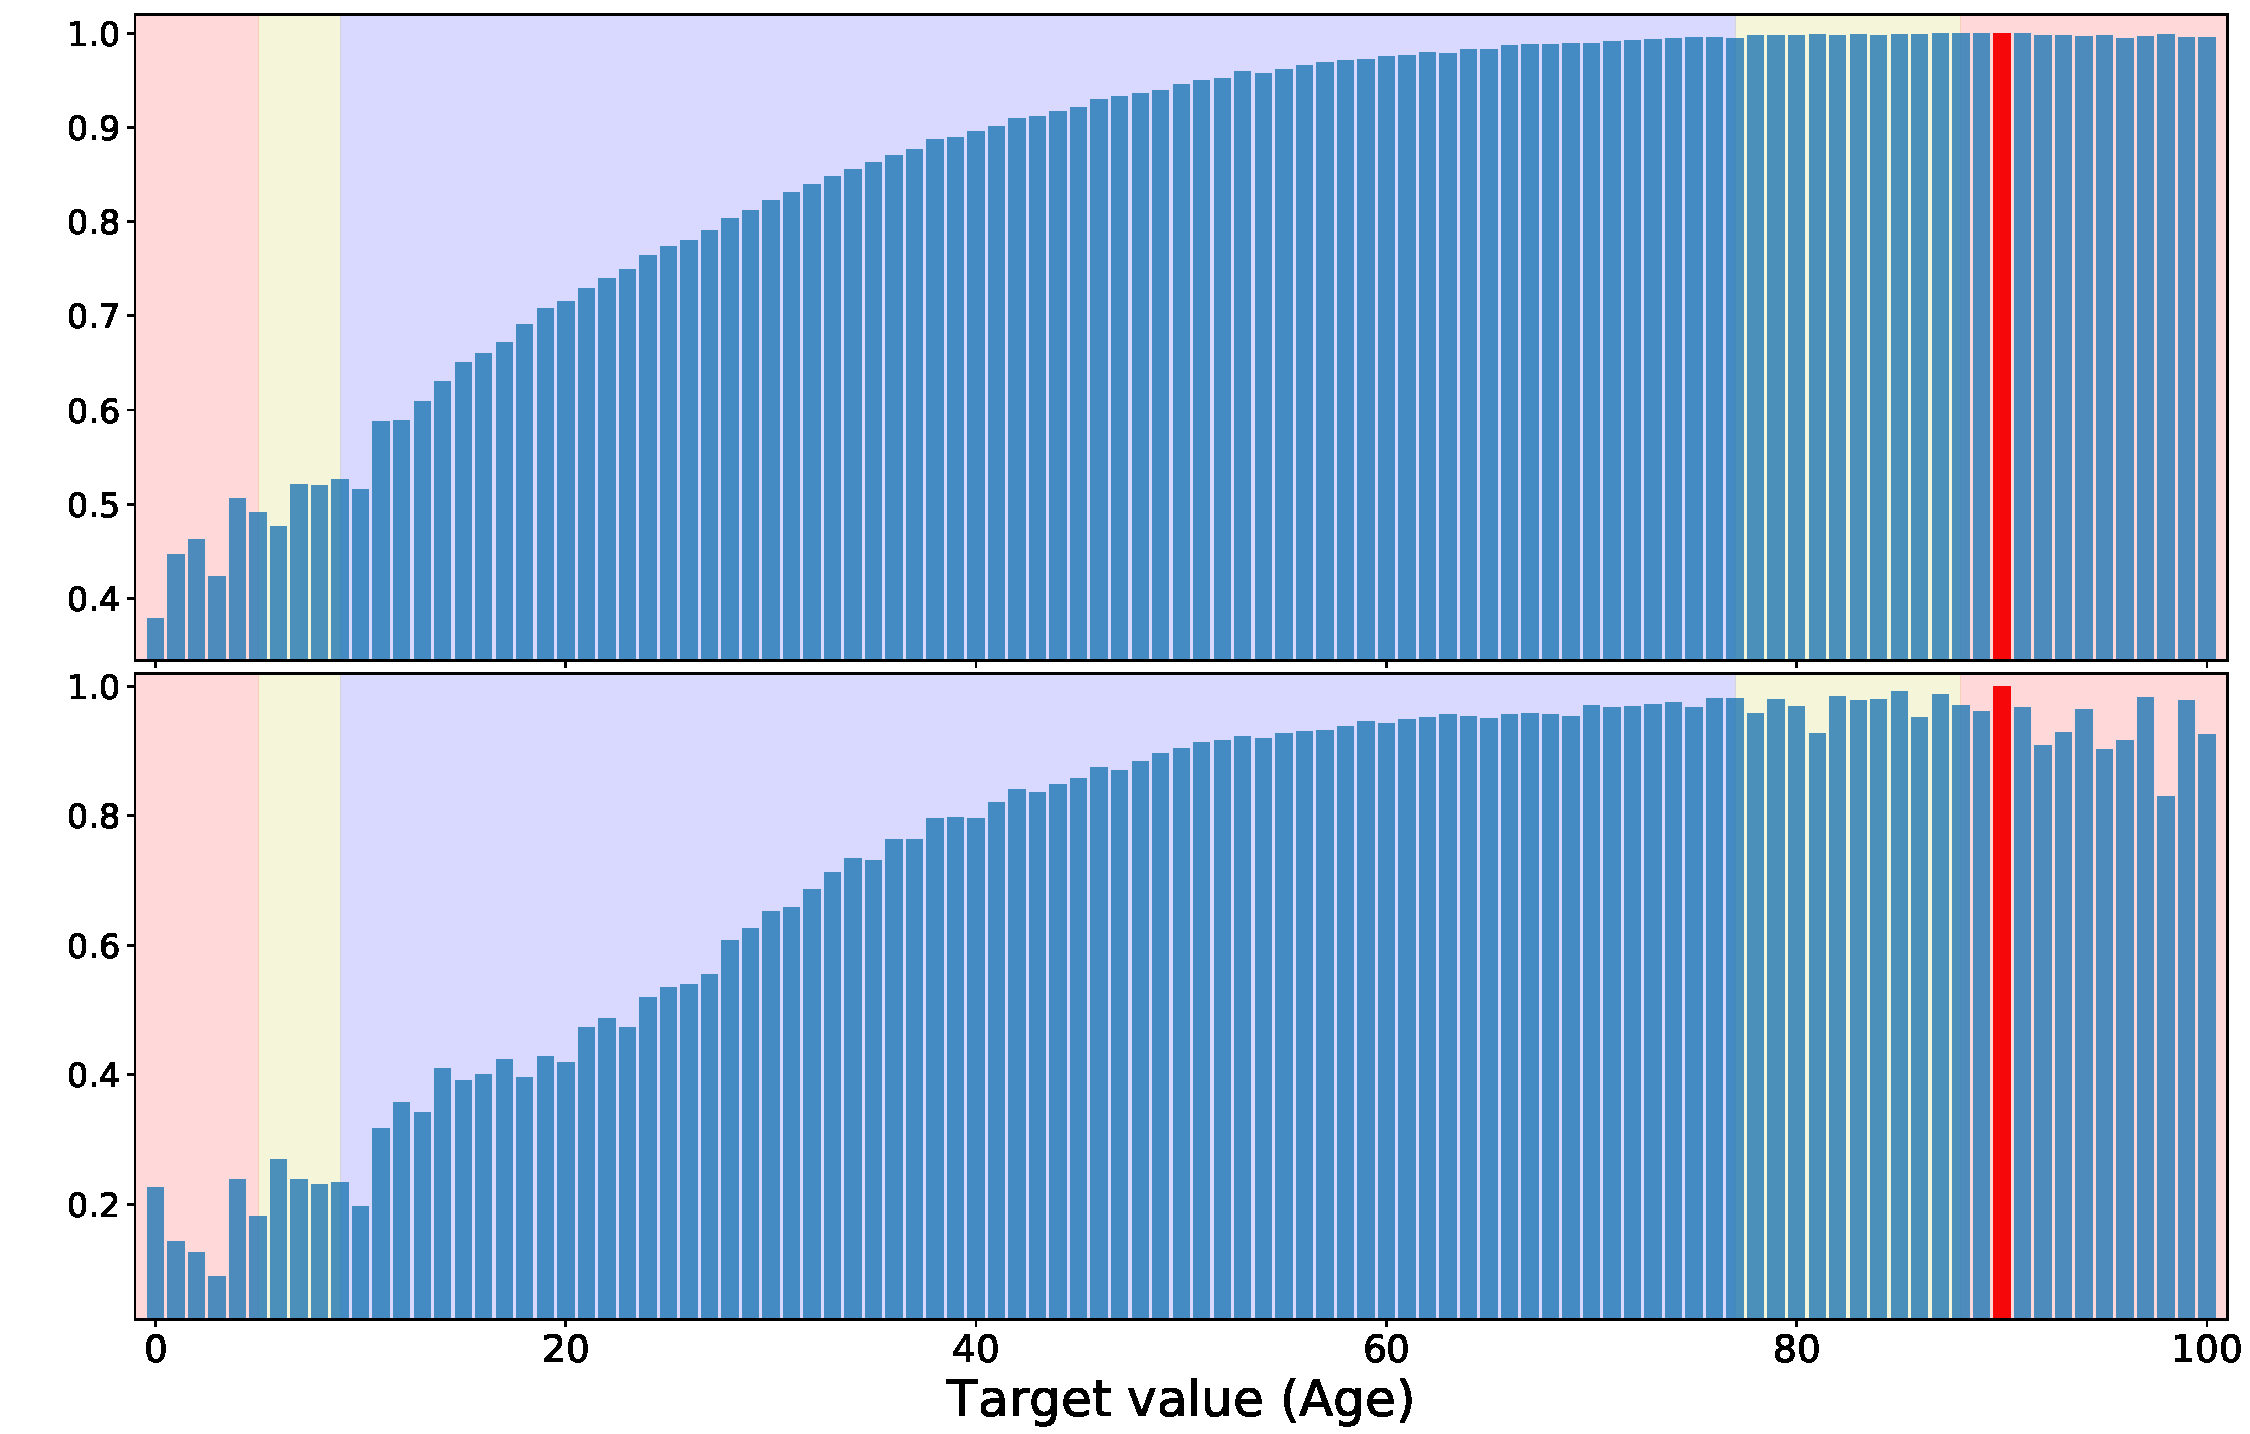
\includegraphics[width=\linewidth]{images/feat_sim_fds_ours_90.pdf}
			\caption{FDS}
		\end{subfigure}
		%\caption{}
	\end{figure}
	\begin{itemize}
		\item FDS improves feature statistics calibration:
		\begin{itemize}
			\item High similarity only in neighbourhood
			\item Gradually decreasing similarity as the target becomes smaller or larger
		\end{itemize}
	\end{itemize}
	\credit{Image}{yang2021delving}
\end{frame}

\begin{frame}{Change of feature statistics w.r.t. epoch}
	\begin{figure}[h]
		\begin{subfigure}{0.48\textwidth}
			\begin{tikzpicture}
				\node[above=0.95em, right=1.5em] at (current page.west)
				{
					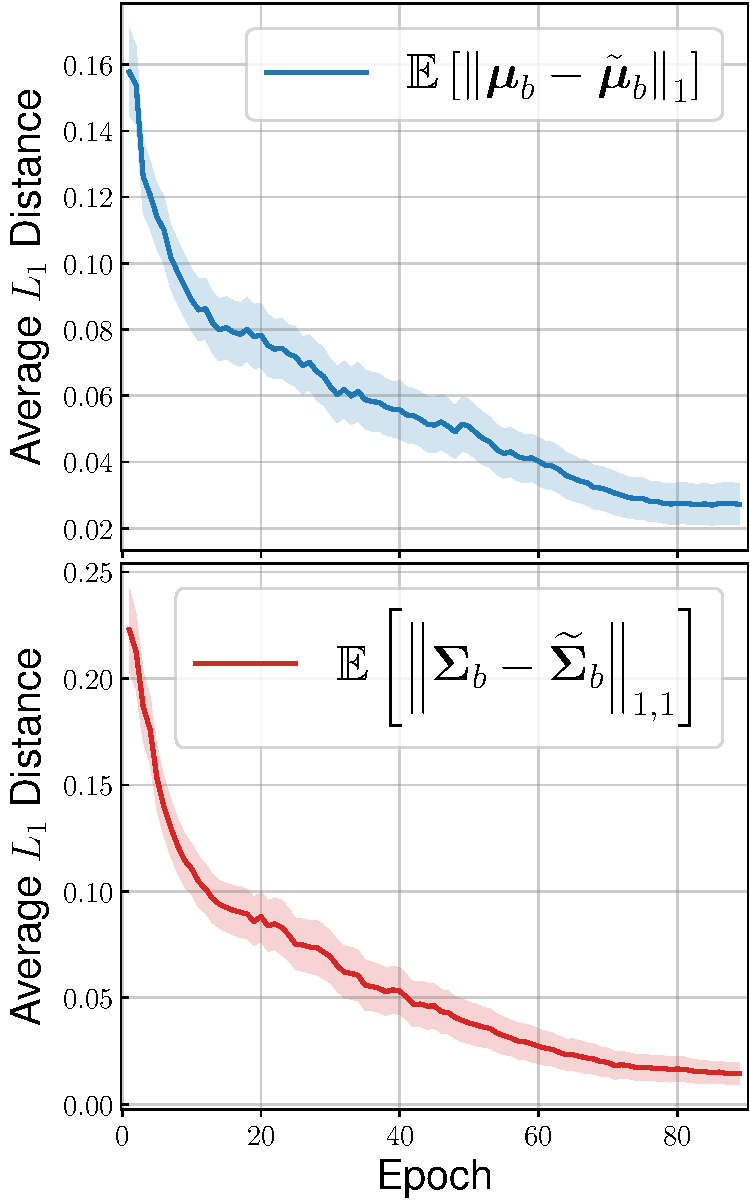
\includegraphics[trim={0 28.5em 0 0},clip,scale=0.4]{images/fds_diff_train.pdf}
				};
				\node[below=4.8em, right=1.5em] at (current page.west)
				{
					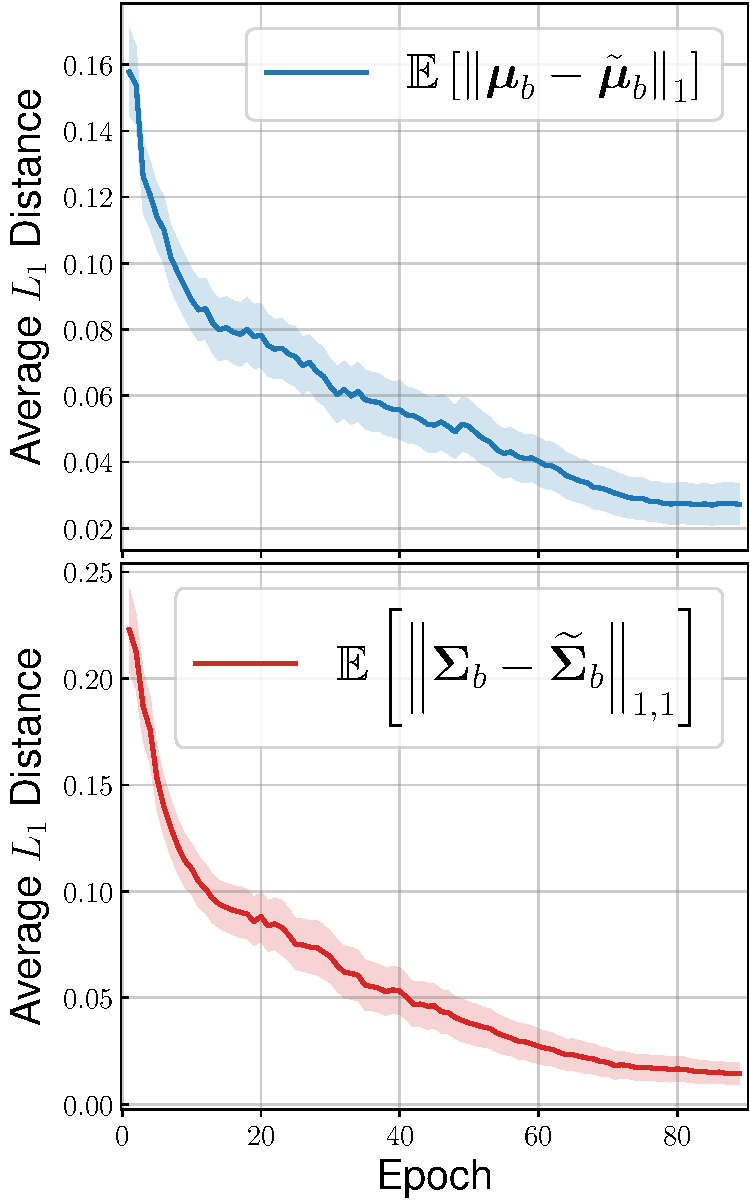
\includegraphics[trim={0 0 0 49.2em},clip,scale=0.4]{images/fds_diff_train.pdf}
				};
			\end{tikzpicture}
			\caption{Mean}
		\end{subfigure}\hspace{1em}%
		\begin{subfigure}{0.48\textwidth}
			\begin{tikzpicture}
				\node[left=1.5em] at (current page.east) 
				{
					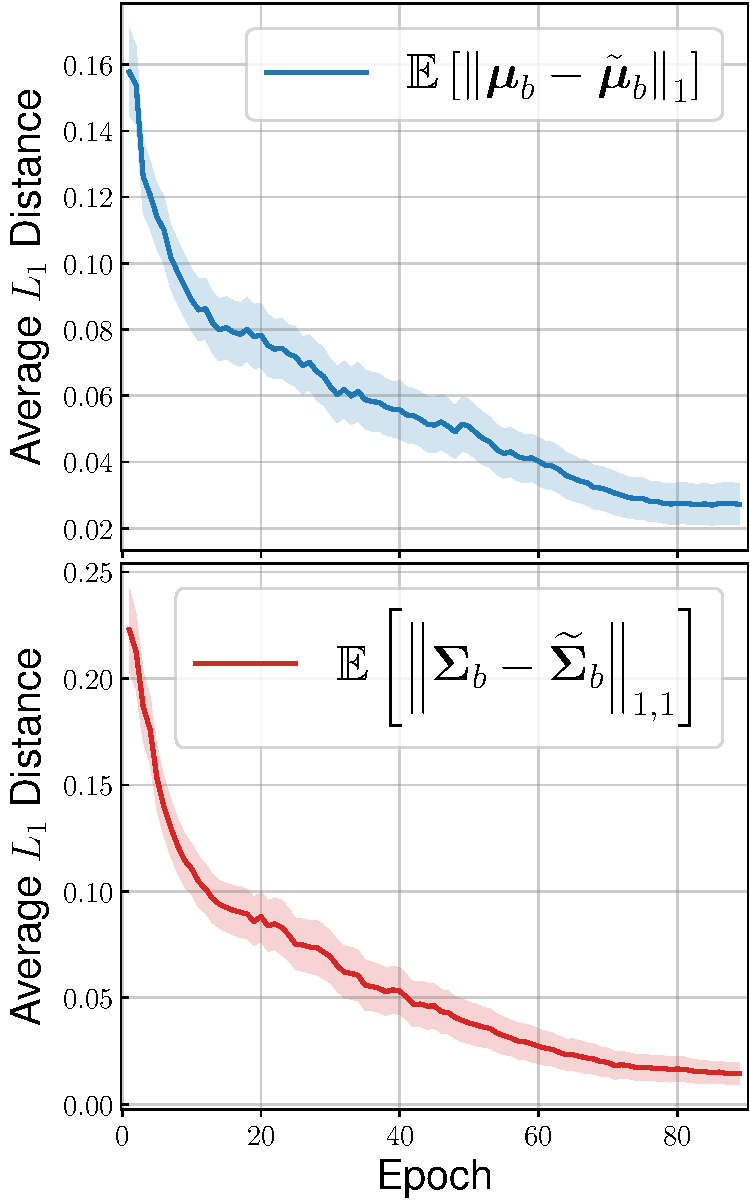
\includegraphics[trim={0 0 0 24.7em},clip,scale=0.4]{images/fds_diff_train.pdf}
				};
			\end{tikzpicture}
			\caption{Variance}
		\end{subfigure}
		%\caption{}
	\end{figure}
	\begin{itemize}
		\item ${\bm{\mu}, \bm{\Sigma}}$: Running mean and variance
		\item ${\bm{\tilde{\mu}}, \bm{\tilde{\Sigma}}}$: Smoothed mean and variance
	\end{itemize}
\end{frame}

\begin{frame}{The FDS Algorithm}
	\begin{figure}[h]
		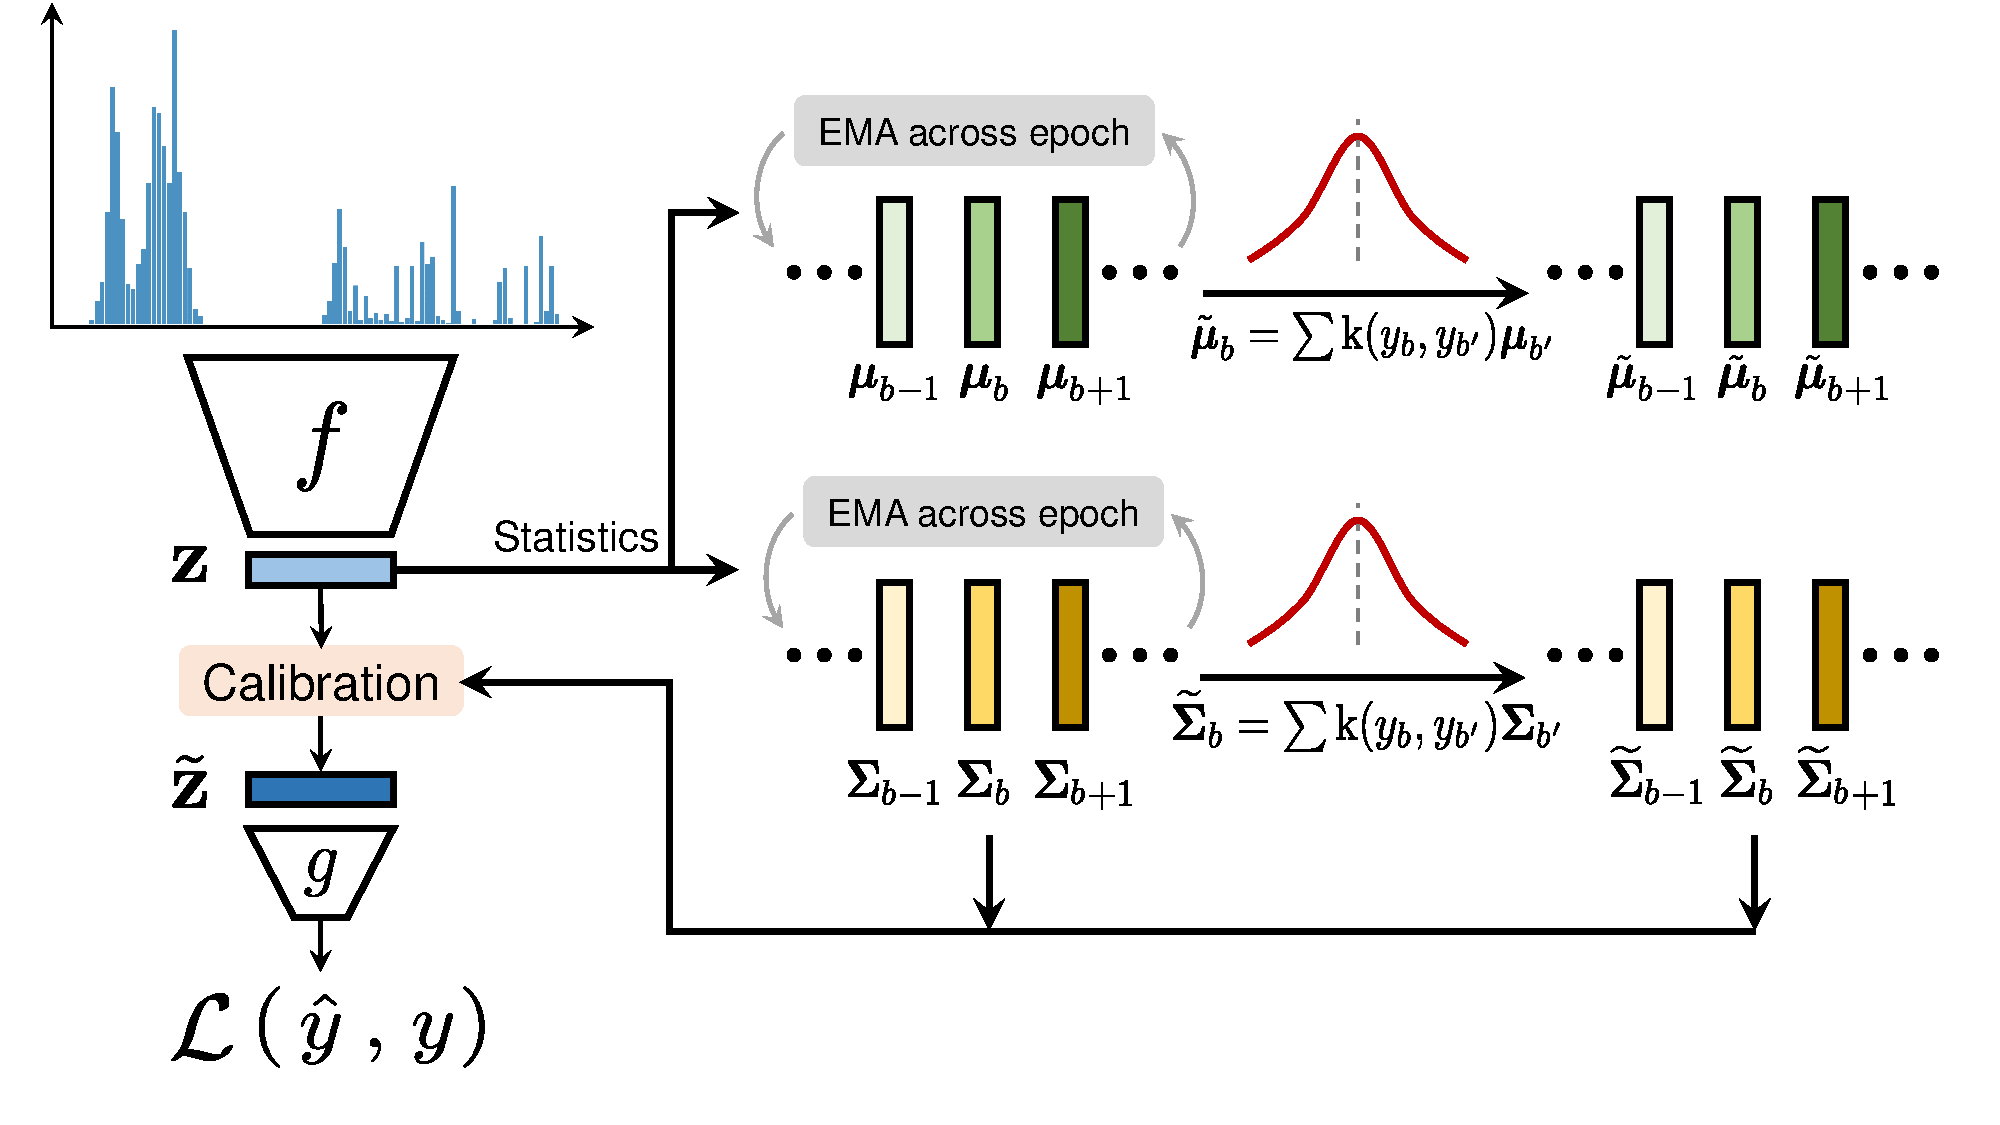
\includegraphics[width=\linewidth]{images/teaser_fds.pdf}
		%\caption{}
	\end{figure}
	\credit{Image}{yang2021delving}
\end{frame}